\chapter{The Teacher who comes first in my mind}\label{chap33}

\Authorline{Balasubramanyam J.}

\authinfo{Formerly, Professor and Head\\
Department of Science and Humanities\\
K S Institute of Technology, Bangalore\\
Presently Senior IIT-JEE Faculty,\\
Base Educational Services Pvt. Ltd., Bangalore\\
j.balasubramanyam@yahoo.co.in}


I met my Guru Professor G. Ramachandran for the first time in September 1983. At that time, I did not know that in the future, I will be recognised as GR's student for life. In my first year as an M.Sc.\ student at Mysore University, he was in-charge of our weekly seminars along with Prof.\ K. S. Puttaswamy. When we were asked to select a topic for the seminar, most of my classmates choose a topic within the syllabus. When I met Prof.\ GR and asked him whether I can choose some topic outside the syllabus, he not only encouraged me to select an emerging topic at that time on the `Quark Model' but also helped me to understand basics of strong interaction at that time. I really struggled a lot and at one point in time with the topic, and I even wanted to change my topic. But he saw to it that I successfully presented my topic. Next two years I and one of my classmates Balasubramanya S. were frequent visitors to his staff room and also to his house at R10, Manasa Gangothri quarters. I can never forget those cherished days in my student life. 

In the second year of our post-graduate studies, we were fortunate to choose ``Theoretical Physics" as an elective, and we were blessed to learn theoretical physics from Prof.\ GR and another great teacher Prof.\ A.V. Gopala Rao. With his blessings and support, I scored the highest marks in Theoretical physics. After my postgraduation, I was interested in doing research under Prof.\ GR and even he was eager to guide me. But due to various reasons, I could not fulfill my dream to work with Prof.\ G.R. at that time, and I started working as a faculty in an engineering college at Chickkaballapur. I could not meet G.R. frequently and pursue my interest in research. However, G.R. stayed in contact with me and he invited me to attend the wedding ceremonies of all his daughters. 

In the year 2000, I left Chickkaballapur and joined another engineering college in Bangalore. After nearly one year I visited Chickkaballapur as an examiner in practical examinations. During the visit, one of my colleagues gave me a postcard that had arrived for me 6 months prior to the visit. It was from Prof.\ G.R.  Prof.\ G.R. wrote to me to let me know that he had moved to Bangalore. He mentioned that he was working at the Indian Institute of Astro Physics (IIAP) in Bangalore. I was excited to learn that I will be able to meet him regularly. As soon as I returned to Bangalore, I rushed to his place. I started meeting him regularly and started renewing my interest in research after a period of nearly 20 years. Eventually, I registered for Ph.D. at Bangalore with Prof.\ A R Ushadevi as a guide and Prof.\ GR as co-guide and successfully completed my Ph.D. in 2009. 

In addition to being a great Physicist, Prof.\ G.R. was a great human being. He never missed an opportunity to help his students whom he felt should not miss out on an opportunity to do research. During my association with him, while working on my Ph.D., I learnt many things in my life in addition to Physics. He used to work harder than me at his age. I still remember that many times, it was usually late in the evening at 11 pm that I left his home after discussion. After reaching my home, it was tough for me to do more work; however, GR usually continued to work late and used to call me as early as 5 am the next day in the morning to tell me about his findings. Many times, I was surprised to learn that G.R. was well informed about different facets of life. At times when he did not discuss physics, he used to talk about many topics including politics, films, spirituality, and other things. Further, I can never forget the hospitality I received at his home. I must say Mrs. Seethalakshmi Ramachandran was very generous and always saw to it that we were not disturbed during our discussions at GR's residence.

I am highly indebted to Prof.\ GR for giving me the tag ``GR's Student". Being his student has also helped me in my professional progress. I have received respect from people at the workplace just by stating that I was GR's student. After I quit working at engineering college, I applied for a faculty position at the BASE (Base Educational Services Pvt Ltd) in 2013. Prof.\ H S Nagaraja (Popularly known as HSN. Fonder of BASE) offered me a job at the BASE as Senior IIT-JEE faculty by considering that I was GR's student, even though I did not have prior experience in IIT-JEE teaching. I owe many things in my life to GR. Wherever I go, whomever I meet, I proudly say I am GR's student. 

One thing which will haunt me for rest of my life is that I could not pay my last respect to him due to lockdown during the COVID-19 pandemic. It gives me immense pleasure to pay my gratitude to him through this article. I would like to mention about my topic of research here: I worked on ``meson production in nuclear reactions". With his guidance and motivation, I could get publications* in reputed journals. 
\vskip 1cm


\centerline{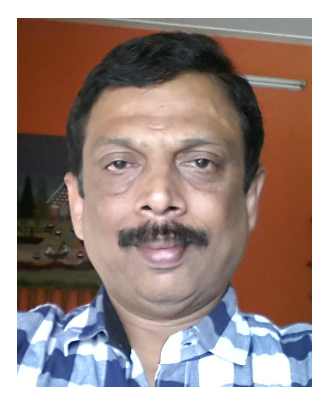
\includegraphics[scale=0.8]{authorsphotos/J_Balasubramanyam.eps}}
\medskip

\noindent
\textbf{Dr.\ J. Balasubramanyam} obtained the M.Sc.\ degree in 1985 from Mysore University and Ph.D. in 2009 from Bangalore University. While doing Ph.D. he was working in the Physics Department, K. S. Institute of Technology, Bangalore, which he joined in 1999. In 2013 he moved from KSIT to BASE Educational Services Pvt.\ Ltd., Bangalore, where he is currently a Professor.

